\documentclass[11pt]{article}
\usepackage[margin=1in]{geometry}
\usepackage{amsmath,amssymb,booktabs,array,graphicx,longtable,algorithm,algpseudocode}
\usepackage[hidelinks]{hyperref}
\usepackage[T1]{fontenc}
\usepackage{lmodern}
\newcommand{\doctype}{Unsubmitted research manuscript}
\newcommand{\docversion}{v0.01}
\newcommand{\docdate}{11 November 2026}
\newcommand{\versiondoi}{not assigned}
\newcommand{\conceptdoi}{not assigned}
\newcommand{\docrepo}{github.com/fsantibanezleal/CAOS\_PhaseFlow}
\newcommand{\headerblock}{\begin{center}\fbox{\parbox{0.94\textwidth}{\small\raggedright
\textbf{\doctype}\quad$\cdot$\quad\docversion, \docdate\quad$\cdot$\quad Licence CC BY 4.0\\
CAOS Research, PhaseFlow open-pit production scheduling\\
Version DOI \texttt{\versiondoi}\quad$\cdot$\quad Concept DOI \texttt{\conceptdoi}\\
Draft for independent review. No Zenodo record has been assigned.\\
Not peer reviewed. Source code and research records: \href{https://\docrepo}{\texttt{\docrepo}}
}}\end{center}\vspace{4pt}}
\title{A State-Conditioned Feasible-Frontier Policy for Open-Pit Scheduling: Design, Feasibility, and Training Evidence}
\author{Felipe Santibáñez-Leal\\ORCID: 0000-0002-0150-3246}
\date{}
\begin{document}
\maketitle
\headerblock
\begin{abstract}
Multi-period open-pit production scheduling couples discounted block value with precedence and period-specific resource limits. A constructive topological scheduler can maintain feasibility while a priority rule chooses among currently available blocks, but static rankings do not respond to the partial schedule or residual capacity. This paper describes a graph-conditioned actor-critic policy that scores precedence-ready, resource-feasible blocks from the current scheduling state. Two explicit stop actions permit unused capacity and partial plans; a separate validator recomputes precedence, capacities, and discounted net present value from the emitted assignments. The implementation uses a fixed graph encoder, state-conditioned actor and critic, masked proximal policy optimization, seed- and family-disjoint generated instances, and external checkpoints. Five CPU-capped members completed under the frozen protocol. Their final training-validation means were between 0.000000 and 0.002744 normalized net present value, without paired baselines. A post-selection replay on the same validation partition found nonempty schedules in 49 percent of 200 cases, a median normalized objective of zero, and zero median positive-value coverage. The one-shot 500-case test evaluation then lost its outputs during final serialization; the partition is consumed and no test metric is available. These results establish neither comparative quality nor generalization. We present the method and its evidence boundary so the design can be examined without turning feasibility into a performance claim.
\end{abstract}
\noindent\textbf{Keywords:} open-pit mine planning, production scheduling, graph policy, constrained reinforcement learning, feasibility masking, reproducibility

\section{Introduction}
Open-pit production scheduling assigns selected blocks to time periods while respecting slope precedence, mining capacity, processing capacity, and a discounted economic objective. In a block model, one extraction decision can unlock other blocks and consume capacity needed by competing opportunities. A rule that orders blocks once before scheduling may therefore ignore the value of the partial plan and the resources remaining in the current period. Conversely, solving the full mixed-integer model at every interaction can make exploratory analysis expensive. The design question addressed here is whether a learned sequential policy can use current scheduling state to choose among legal next actions while retaining a transparent, independent feasibility check.

The policy operates on a fixed precedence graph. Each node carries normalized block and geological features; edges encode immediate predecessor relations. At each step the state also records the period, residual resources, accumulated discounted value, and the size of the feasible frontier. The actor scores eligible blocks jointly with this state. An action mask removes any block that violates precedence or exceeds a remaining resource capacity. A stop-period action advances the horizon, and a stop-schedule action returns a partial plan. This formulation is distinct from a learned block ranker: two instances with identical static node features can yield different admissible actions because their partial schedules differ.

The method is a research implementation, not an operational recommendation system. Its schedule decoder is designed to preserve modeled constraints, while its learned objective quality remains an empirical question. This distinction matters because a feasible empty schedule has zero capacity violations but zero production coverage. We therefore report feasibility separately from selected blocks, positive-value coverage, discounted net present value (NPV), runtime, memory, and benchmark comparisons. A constraint check cannot stand in for economic performance, and a small positive normalized NPV cannot be interpreted without a matched baseline and uncertainty.

This study has three aims. First, it specifies the scheduling state, graph encoder, action mask, reward, training update, and independent schedule validation in enough detail for review. Second, it records exactly what the capped implementation did on the predeclared generated training and validation design, including the early stopping behavior, selected checkpoints, and weak validation outcomes. Third, it explains why the single synthetic test attempt cannot support a result: evaluation completed in memory but serialization failed before per-case outputs were persisted. The consumed split is not reopened here, and product cases remain unopened. We do not infer a test statistic from training logs or reconstruct a result from an incomplete run record.

The contribution is thus methodological and reproducibility-oriented. We provide an explicit state-conditioned masked policy for a finite-horizon precedence-constrained schedule, a deterministic ensemble replay path, and an independent constraint and objective validator. The study also reports a negative training outcome and a release-blocking evaluation failure. It does not claim that the policy improves on greedy construction, expected-time ordering, published scheduling heuristics, or exact optimization. No application selector exposes the checkpoints, and no model weights are included in this repository. Figure~\ref{fig:decision-cycle} summarizes the decision loop; the held-out boundary and the failure path are shown separately in Figure~\ref{fig:evidence-boundary}.

\section{Related work}
The scheduling problem rests on graph closure and precedence-constrained optimization. Lerchs and Grossmann formulate ultimate pit design as a maximum-value pit problem, and Picard characterizes maximum closure with network-flow structure \cite{lerchs1965,picard1976}. Hochbaum surveys closure models and their algorithmic implications \cite{hochbaum2004}. These results motivate the precedence graph and pit-limit construction, but an ultimate pit is not a period schedule: period assignment introduces resource limits and discounting that a closure optimum alone does not resolve.

Open-pit scheduling formulations range from block-sequencing integer models to relaxation-based and constructive methods. Johnson's production scheduling formulation and later reviews describe the interaction of extraction order, capacity, and economic value \cite{johnson1968,newman2010,lambert2014,meagher2014}. Branch-and-cut can target the integer formulation, while critical-multiplier methods derive fractional expected extraction times and upper bounds from maximum-closure subproblems \cite{caccetta2003,chicoisne}. The Bienstock-Zuckerberg algorithm scales large precedence-constrained LP relaxations, and mining applications compare those bounds with feasible schedules \cite{bienstock,munoz2017}. Disaggregation, aggregation, and large mixed-integer methods provide different trade-offs between formulation size, bound quality, and runtime \cite{boland2009,jelvez2016,askari2010}. These are relevant comparators because they distinguish a concrete feasible schedule from a mathematical certificate.

Constructive mine-planning heuristics exploit precedence to build feasible plans incrementally. Gershon's successor-cone weighting values blocks partly through the opportunities they unlock; expected-time TopoSort orders eligible blocks using fractional relaxation signals \cite{gershon,chicoisne}. A sliding-window heuristic optimizes a restricted portion of the horizon and can reconsider nearby decisions at additional computational cost \cite{cullenbine2011}. MineLib provides benchmark formulations and instances, while later corrections to the library show why case provenance and exact formulation interpretation matter \cite{espinoza2013,jelvez2018}. PhaseFlow uses these approaches as implemented comparators in its existing benchmark line, but the current state-conditioned policy has no completed paired comparison against them.

Destination choice, blending, stockpiling, and geological uncertainty enlarge the decision state beyond fixed-destination CPIT. Published linear models address stockpile inventory and blending, and degradation models account for changing material quality \cite{moreno2017,rezakhah2020blend,rezakhah2020degrade}. Stochastic and robust mine schedules represent uncertain supply, reserve uncertainty, and recourse decisions \cite{ramazan2013,goodfellow2016,lamghari2012,lamghari2016}. The policy in this paper does not model stockpile inventory, reclaim, blending recourse, equipment assignment, or stochastic geological realizations. It schedules a deterministic generated graph with the resource arrays declared in the contract. Inference on that contract does not imply coverage of the omitted models.

Reinforcement learning has been applied to mine-complex scheduling and planning updates, including tree-search and actor-critic approaches \cite{kumar2021,carvalho2023}. Graph neural networks have also been used for resource-constrained project scheduling, where precedence structure and a changing feasible set are central \cite{teichteil2023,zhao2022}. Proximal policy optimization (PPO) constrains policy updates through a clipped surrogate objective, and Adam provides an adaptive first-order optimizer \cite{schulman2017,kingma}. Large-neighborhood search supplies a non-learning alternative for long-term mine planning \cite{blom}. These studies motivate graph representation, sequential action, and learning baselines; they do not establish that the present policy generalizes to mine operations or beats the PhaseFlow comparators. Their decision horizon, objective, information updates, and feasibility decoder differ, so citation is not a substitute for a matched product run.

The design choices made here address gaps between a graph policy and a mine schedule. The graph network encodes static precedence structure once per instance, while a small state vector changes after each assignment. The mask is a hard decoder rule rather than a penalty learned from reward. An independent validator checks the final extracted assignment list instead of trusting the network's logits, training reward, or action mask. This combination borrows the graph representation and policy-gradient machinery from scheduling research but retains the explicit capacity and precedence semantics of the underlying CPIT model. The result is a concrete algorithmic hypothesis to test, not a claim of novelty across all mining reinforcement learning.

The relevant comparison dimensions are summarized in Table~\ref{tab:related-methods}. The table distinguishes implemented families by their decision signal and certificate. It makes clear that the policy's current evidence is not comparable to completed product results because it has no paired test values. Figure~\ref{fig:decision-cycle} and Figure~\ref{fig:mask-example} show how the proposed decoder uses the same constraint structure while allowing a learned score to affect selection.
\begin{table}[ht]
\centering\small
\caption{Scheduling families differ in decision signal, state dependence, feasibility mechanism, and evidence presently available in PhaseFlow.}\label{tab:related-methods}
\begin{tabular}{>{\raggedright\arraybackslash}p{0.17\textwidth}>{\raggedright\arraybackslash}p{0.20\textwidth}>{\raggedright\arraybackslash}p{0.27\textwidth}>{\raggedright\arraybackslash}p{0.22\textwidth}}
\toprule Family & Decision signal & Feasibility or certificate & PhaseFlow evidence \\
\midrule
Greedy TopoSort & Static block value & Eligible-frontier construction & Existing baseline results \\
Expected-time TopoSort & Fractional extraction-time signal & Precedence-safe construction and bound comparison & Existing baseline results \\
Sliding window & Restricted-horizon integer re-solve & Model constraints plus schedule validation & Existing baseline results \\
Graph-conditioned policy & Current state and graph context & Hard action mask plus independent validator & Training validation only; no paired test \\
Exact scheduling model & Full integer objective & Solver feasibility and proof status & Case dependent; no policy comparison yet \\
\bottomrule
\end{tabular}
\end{table}

\section{Problem formulation}
Let $B$ be the blocks in an instance, $T$ the finite number of periods, $R$ the resource set, and $A\subseteq B\times B$ the directed precedence arcs. An arc $(i,j)$ means block $i$ must be extracted no later than block $j$. Let $v_i$ be the fixed-destination value of block $i$, $a_{ri}\geq0$ its use of resource $r$, $c_{rt}\geq0$ the available capacity of resource $r$ in period $t$, and $\eta\geq0$ the discount rate. A schedule is a set of block-period assignments $S\subseteq B\times\{0,\ldots,T-1\}$, with at most one assignment per block. Its discounted objective is
\begin{equation}
V(S)=\sum_{(i,t)\in S}\frac{v_i}{(1+\eta)^{t+\delta}},\qquad \delta\in\{0,1\},
\label{eq:objective}
\end{equation}
where $\delta$ is fixed by the case contract to select its period-one convention. The objective convention is an input, never inferred from a chart. Equation~\ref{eq:objective} is recomputed by the validator from assignments after inference.

For each period, resource use is $u_{rt}(S)=\sum_{(i,t)\in S}a_{ri}$. Feasibility requires $u_{rt}(S)\leq c_{rt}$ for all $r,t$. If block $j$ is assigned to period $t_j$, every predecessor $i$ must also be assigned and satisfy $t_i\leq t_j$. The schedule may be partial: an unscheduled block is not assigned a default period and cannot contribute value or coverage. This is important because the policy contains a stop-schedule action; a feasible partial schedule is not a complete plan.

At decision step $k$, the state is $s_k=(t_k,y_k,q_k,z_k)$, where $t_k$ is the current period, $y_k$ is the vector of assigned periods with a sentinel for unassigned blocks, $q_k$ is residual capacity in the current period, and $z_k$ contains the normalized accumulated value and feasible-frontier size. The graph is $G=(B,A)$ with node-feature matrix $X\in\mathbb R^{|B|\times d}$. The admissible block set is
\begin{equation}
\mathcal F(s_k)=\{i\in B:y_{ki}=\bot,\; j\in\operatorname{pred}(i)\Rightarrow y_{kj}\leq t_k,\; a_{ri}\leq q_{kr}\;\forall r\in R\}.
\label{eq:frontier}
\end{equation}
Equation~\ref{eq:frontier} combines precedence readiness and all current resource constraints. The two stop actions are always admissible. A stop-period action advances to the next period unless the horizon is complete; a stop-schedule action terminates immediately. The action space therefore has $|B|+2$ indices and a Boolean mask with true entries only for $\mathcal F(s_k)$ and the stop actions.

We distinguish three properties throughout. Constraint feasibility is whether the assignment list satisfies the encoded inequalities and precedence. Coverage is the fraction of total tonnage or positive block value assigned. Schedule quality is $V(S)$ and its paired difference or ratio to a baseline. A valid schedule can have low coverage and low NPV, as the validation diagnostic later demonstrates. These are not interchangeable outcomes. The problem scope excludes destination recourse, inventory, blending, uncertain realized grade, and equipment routing; such decisions change the mathematical state and cannot be smuggled into node features without a corresponding contract.

\section{Proposed method}
\label{sec:proposed-method}
The method has four stages: construct a fixed graph representation, encode it with message passing, score legal actions from the dynamic schedule state, and independently validate the final schedule. Figure~\ref{fig:architecture} gives the computation graph, and Figure~\ref{fig:mask-example} illustrates how an action can be removed for either precedence or resource reasons. The actor does not receive a list of future test labels, a case identifier, or a product-specific lookup key. The input feature contract contains seven node variables: normalized value, normalized tonnage, plant-use fraction, normalized grade, depth fraction, predecessor count, and successor count. Train-only means and scales are stored in each checkpoint and applied identically at evaluation.

\subsection{Graph and dynamic state encoding}
The initial node embedding is $h_i^{(0)}=\operatorname{ReLU}(W_0\tilde x_i+b_0)$, where $\tilde x_i$ is the standardized feature row. At each message-passing layer $\ell\in\{0,1\}$, the network computes the mean incoming and outgoing neighbor embeddings. It concatenates those two summaries with the node's current embedding and applies an affine transformation and ReLU:
\begin{equation}
h_i^{(\ell+1)}=\operatorname{ReLU}\left(W_\ell[h_i^{(\ell)}\Vert m_{i,\mathrm{in}}^{(\ell)}\Vert m_{i,\mathrm{out}}^{(\ell)}]+b_\ell\right).
\label{eq:message}
\end{equation}
The graph encoder is computed once per instance because precedence edges and standardized block features do not change during an episode. Equation~\ref{eq:message} uses mean aggregation, so the magnitude of a sum does not grow mechanically with node degree. It does not guarantee invariance to graph-family shift or preserve all graph structure; two iterations expose each node only to a limited neighborhood before the policy acts.

The node contract is intentionally small and dimensionless. For raw feature $x_{ij}$ of feature $j$ on block $i$, the trainer estimates $\mu_j$ and a positive scale $\sigma_j$ using training rows only. The deployed transformation is
\begin{equation}
\tilde x_{ij}=\frac{x_{ij}-\mu_j}{\max(\sigma_j,\epsilon)},\qquad \epsilon>0,
\label{eq:normalization}
\end{equation}
where the scale floor is part of the serialized normalizer contract. Validation and test graphs reuse these frozen training statistics. Re-estimating means from a held-out partition would leak distribution information and make a checkpoint depend on the evaluation set. The run record hashes both the feature list and the normalization payload, so feature reordering, adding a proxy, or changing the scale procedure defines a different method snapshot.

Value and tonnage are normalized by the instance scale; grade is bounded and scaled; depth expresses relative vertical position; predecessor and successor counts are normalized to avoid making raw graph size the only signal. Plant-use fraction describes the generated capacity regime. These variables are not independent: grade and value may share construction inputs, while depth can correlate with predecessor count. Their inclusion is a modeling choice, not evidence that the learned representation isolates a causal effect. A feature audit must test forbidden identifiers and compare the transformed vector against the canonical pipeline implementation. It must also test zero variance, nonfinite input, changed feature order, and a held-out graph whose raw feature lies outside the training range. The current feature contract rejects invalid scale and nonfinite values but does not claim robust extrapolation beyond the generated support.

The current graph actor has two message-passing layers of width 64 and a shared actor with one 64-unit hidden layer. This shares parameters across blocks: the actor evaluates the same function at every node rather than assigning a separate learned head to every block index. The critic pools node embeddings by mean and combines that pooled summary with the state. Mean pooling limits direct sensitivity to block count, yet it can blur distinct graph structures that share average embeddings. A larger receptive field or attention mechanism might represent more distant precedence effects, but it would also add parameters and training burden. Neither alternative is justified by the present negative validation result; architectural changes require a separately versioned experiment, not a post-hoc patch followed by reuse of the consumed test.

The dynamic state vector records normalized period index, one residual-capacity fraction per resource, normalized accumulated discounted value, and frontier size divided by block count. For candidate block $i$, the actor concatenates $h_i^{(2)}$ with this vector and emits a scalar logit. A separate stop actor emits two logits from the state. The critic combines mean-pooled node embeddings with the state and estimates the value of the current state. These heads share neither a hand-coded priority score nor a scalar reward model. Their parameters are updated by PPO from sampled finite-horizon episodes.

For resource $r$ in the current period, residual capacity is recomputed from assignments rather than incrementally trusted as an independent source of truth:
\begin{equation}
q_{kr}=c_{r,t_k}-\sum_{(i,t_k)\in S_k}a_{ri},\qquad \rho_{kr}=\begin{cases}q_{kr}/c_{r,t_k},&c_{r,t_k}>0,\\0,&c_{r,t_k}=0.\end{cases}
\label{eq:residual}
\end{equation}
Equation~\ref{eq:residual} defines the resource coordinates supplied to the network and the feasibility test uses the unnormalized $q_{kr}$. A capacity of zero is not treated as infinite capacity: a block using positive resource is inadmissible. Recalculation makes the state auditable but adds work proportional to assignments at each transition; an optimized accumulator could be introduced only if parity tests proved it identical for every period and edge case.

\subsection{Masking and state transition}
The policy uses the mask derived in Equation~\ref{eq:frontier} before selecting an action. If $\ell_i(s)$ is the actor logit for block $i$, the masked distribution is
\begin{equation}
\pi_\theta(i\mid s,G)=\frac{\exp(\ell_i(s))}{\sum_{j\in\mathcal F(s)\cup\{\mathrm{stopP},\mathrm{stopS}\}}\exp(\ell_j(s))},\qquad i\in\mathcal F(s),
\label{eq:masked-policy}
\end{equation}
with inadmissible block logits set to negative infinity before normalization. Equation~\ref{eq:masked-policy} prevents the sampler from selecting a block that the current state cannot legally accept. It is not a proof that the final schedule is valid: errors in state updates, indexing, discount conventions, or exported assignments could still violate the model. The validator therefore reconstructs resource use and predecessor timing from the output assignments and fails closed if any condition is broken.

When a block is assigned in period $t$, the transition appends $(i,t)$, updates residual capacity and accumulated value, and recomputes the frontier. When stopP is selected, the period increments and residual capacities reset to the next row of the case matrix. When stopS is selected, the episode terminates with a partial schedule. At the final period, stopP also terminates. An empty frontier leaves both stop actions available, preventing an invalid forced selection. These transitions are implemented explicitly; the decoder does not repair an invalid network action silently.

The schedule state is derived from the assignment history and case matrices, rather than directly from the actor's hidden memory. Let $S_k$ denote the assignment set after $k$ actions and $C_t$ the capacity vector in period $t$. For a block $i$, the residual check is the componentwise condition $a_i\preceq C_t-\sum_{j:(j,t)\in S_k}a_j$. The notation $\preceq$ means that every resource coordinate satisfies the inequality. This avoids an aggregate scalar penalty that could hide a mining-capacity violation behind spare processing capacity. If a new block exactly fills one resource, equality is admissible within the numeric tolerance used by the validator; if floating representation pushes use above the limit by more than tolerance, validation fails. The same tolerances are specified in tests and are not learned parameters.

The two stop actions have different state transitions and are not interchangeable labels. stopP closes the current period and makes the next period's capacity available; it does not promise that a block will be assigned there. stopS closes the entire episode, even if later periods remain. The environment records a termination reason so that the exported schedule can distinguish a deliberate early stop from reaching the horizon. Coverage is computed after validation from the assigned block indices:
\begin{equation}
\operatorname{Cov}_{+}(S)=\frac{\sum_{i\in S}\max(v_i,0)}{\sum_{i\in B}\max(v_i,0)},\qquad
\operatorname{Cov}_{T}(S)=\frac{\sum_{i\in S}w_i}{\sum_{i\in B}w_i},
\label{eq:coverage}
\end{equation}
where $w_i$ is tonnage. A zero denominator is handled as an undefined-support case in the result contract rather than silently interpreted as complete coverage. Equation~\ref{eq:coverage} does not influence the PPO reward in the frozen run; it is reported to reveal when the policy stops too early.

\subsection{Reward, policy update, and inference}
For a block assignment, the reward is its discounted value divided by the maximum of total absolute instance value and a small positive constant. Stop actions yield zero immediate reward. The training objective maximizes the expected sum of normalized rewards; it does not include a separate reward for extracting all positive-value material. The design therefore allows the policy to stop early if its value estimate favors stopping. This may be rational under a learned objective model yet is unacceptable operationally when the resulting coverage is negligible, which is why coverage is measured explicitly.

PPO uses the clipped probability ratio with generalized advantage estimates, a learned value baseline, entropy regularization, and gradient-norm clipping. For old policy $\pi_{\theta_0}$, advantage estimate $\hat A_k$, ratio $r_k(\theta)=\pi_\theta(a_k\mid s_k)/\pi_{\theta_0}(a_k\mid s_k)$, and clip width $\epsilon$, the actor term is
\begin{equation}
L^{\mathrm{clip}}(\theta)=\mathbb E_k\left[\min\left(r_k(\theta)\hat A_k,\operatorname{clip}(r_k(\theta),1-\epsilon,1+\epsilon)\hat A_k\right)\right].
\label{eq:ppo}
\end{equation}
The critic minimizes squared return error; entropy encourages exploration during training. The implementation uses learning rate $3\times10^{-4}$, clip width $0.2$, generalized-advantage parameter $0.95$, entropy coefficient $0.01$, value coefficient $0.5$, ten update epochs, and a maximum gradient norm of $0.5$. These are fixed experimental parameters, not values selected from the consumed test partition.

For deterministic evaluation, the five selected members emit action logits for the same observation. The logits are averaged, inadmissible actions are masked, and the maximum legal action is selected with deterministic index tie-breaking. The graph embeddings are cached for each member within an episode. Inference enforces a per-instance time cap; a timeout becomes an explicit failed result rather than a silent fallback to another method. Figure~\ref{fig:decision-cycle} traces this loop, while Figure~\ref{fig:evidence-boundary} separates training, validation, one-shot test, and product-case evaluation.

The deterministic ensemble uses arithmetic averaging of member logits before masking, not majority voting or averaging schedule outputs. This choice means one large-magnitude member can affect the aggregate; it is fixed by the implementation contract. Every member receives the same graph, feature normalizer, current assignment state, and action mask, but each has independent learned parameters. Action selection is a global argmax over all admissible blocks and the stop logits. Ties are resolved deterministically by canonical action index. These details matter for reproducing traces: sampling during evaluation would create an additional random variable and make repeated results depend on the random stream, while averaging already-decoded schedules would not define a coherent sequential decision rule.

The inference complexity is dominated by graph encoding and repeated actor scoring. For $n$ blocks, $m$ precedence edges, hidden width $h$, and $K$ selected models, one message-passing layer costs $O((n+m)h^2)$ with dense transforms and neighbor aggregation. Two layers are computed once. Each assignment step scores up to $n$ candidate nodes for each of $K$ models, so a loose upper bound over at most $n$ assignments is $O(Kn^2h)$ in actor evaluation, in addition to repeated frontier computation. The current implementation favors a simple, transparent baseline and enforces a runtime cap; it does not claim asymptotically optimal incremental frontier updates. A runtime result must therefore include graph size, edge count, assignment count, hardware, and whether encoding or replay is timed.

\begin{algorithm}[ht]
\caption{Deterministic masked ensemble schedule generation with independent final validation.}\label{alg:policy}
\begin{algorithmic}[1]
\Require Instance $(G,X,a,c,v,\eta)$ and five frozen actor-critic checkpoints
\Ensure Validated complete or partial schedule, or an explicit failure
\State Standardize $X$ with the checkpointed train-only feature contract
\State Encode $G$ once for each checkpoint; initialize empty assignments and period $t\gets0$
\While{the episode has not terminated}
  \State Build state $s$ and admissible set $\mathcal F(s)$ from precedence and residual capacity
  \State Average the five actor logits and two stop logits; mask inadmissible block actions
  \State Select the maximum-logit admissible action with deterministic tie-breaking
  \If{the action assigns block $i$}
    \State Append $(i,t)$; update resource use and discounted objective
  \ElsIf{the action stops the period}
    \State Advance $t$ or terminate if the horizon is complete
  \Else
    \State Terminate with an explicitly partial schedule
  \EndIf
\EndWhile
\State Recompute precedence, capacities, objective, tonnage coverage, and value coverage from assignments
\State \Return the result only if independent validation succeeds
\end{algorithmic}
\end{algorithm}

\subsection{Independent schedule validation}
The final validator receives the original instance and the emitted assignment sequence, not the model's accumulated reward. It rejects duplicate block indices, out-of-range block or period values, resource overuse, missing predecessors, and precedence inversion. It then recomputes discounted NPV from the per-block values and the case's period convention. Tonnage and positive-value coverage are calculated from the selected block indices and checked against finite nonnegative input arrays. This check is independent of the action distribution and is invoked by the policy environment before a result object is returned.

The training callback calls the environment's result method at the end of every validation episode. Therefore the \texttt{all\_feasible} training field is backed by the validator: an infeasible result raises and is not counted as a completed validation summary. The field means only that all returned schedules passed the encoded constraints. It does not assert full extraction, useful value coverage, economic quality, or a comparison with another method. A valid empty schedule is feasible. The separation between this validator and objective evaluation is deliberate and is discussed in Section~\ref{sec:theory}.

The validator checks the emitted assignment sequence rather than trusting cached state. It reconstructs a period-by-resource usage matrix from zero, counts each block once, and then verifies that every assigned block has all required predecessors in the same or an earlier period. This catches defects that can occur when an action mask is correct at decision time but an export path changes block indices or periods. It also detects a reward bookkeeping error if the recomputed NPV differs from the transition reward sum beyond the declared floating tolerance. Validation is fail-closed: it returns no schedule metrics after a structural failure, and the evaluator retains the failure reason rather than substituting an objective from the policy's critic. The current v4 callbacks completed all 200 scheduled validation rows for each checkpoint without a constraint exception, so their feasibility flag is supported by this path. That fact is still narrower than evidence of a useful schedule, as demonstrated by the separate coverage replay.

\section{Theory and properties}
\label{sec:theory}
The method has a deterministic feasibility property conditional on correct inputs and implementation. It does not have a corresponding approximation guarantee for NPV. We state these boundaries because a learned policy can have a legal action mask yet make a poor economic choice, and because the validation output contains many empty or nearly empty schedules.

\subsection{Feasibility invariant}
Suppose the initial assignment set is empty and the instance has nonnegative resource coefficients and capacities. At each step, the mask admits a block only if it is unassigned, every predecessor has been assigned in the current or an earlier period, and all of its resource use fits within residual capacity. Assigning such a block preserves uniqueness by the unassigned condition. It preserves precedence because every predecessor is already scheduled no later than the current period. It preserves capacity because the mask checks every resource coordinate against remaining capacity. A stop action adds no block and therefore preserves all three properties. By induction over the finite action sequence, every schedule emitted by a correct transition implementation satisfies the modeled constraints. The proof is an invariant argument about the decoder; it says nothing about whether the implementation matches the argument, which is why adversarial tests and independent final validation remain necessary.

Formally, let $I_k$ mean that after $k$ transitions, each assigned block appears exactly once, every precedence arc into an assigned block has an assigned predecessor at no later time, and all period-resource totals are within capacity. The base case $I_0$ holds because the assignment set is empty and usage is zero. For the inductive step, a stop action leaves $S_k$ unchanged; a period advance moves to an empty capacity row; and a block action is admitted only after the mask verifies uniqueness, predecessor timing, and residual resources. Thus $I_k\Rightarrow I_{k+1}$. The horizon and finite block count bound the number of block actions, while period and schedule stop actions terminate or advance finitely, so the decoder cannot generate an infinite valid episode. This reasoning assumes the graph is acyclic and resource data are finite and nonnegative; those input conditions are validated before policy execution. If they are violated, the premise of the proof fails and no feasibility guarantee follows.

This proposition is valuable because a policy gradient can assign high probability to illegal actions unless the decoder prevents them. A reward penalty would only discourage violations statistically and could still emit an infeasible schedule after training. A hard action mask instead gives a local guarantee for every sampled action under the contract. Yet the guarantee is conditional on the correctness of the frontier computation, capacity arithmetic, and transition state. The independent validator provides a second path over the final list, and adversarial tests target duplicate blocks, missing predecessors, an exactly filled capacity, slight capacity excess, horizon boundaries, and empty frontiers. These tests are implementation evidence; they do not show that the learned choice among legal actions is economically strong.

\subsection{Objective recomputation}
The reward for assigning a block is the same discounted value term used by Equation~\ref{eq:objective}, scaled by a positive instance constant. Summing assignment rewards therefore yields the scaled schedule objective if and only if the period transition, discount exponent, and assignment list agree with the case contract. The validator independently recomputes the unscaled objective. A parity test can compare the accumulated reward multiplied by the scale with this recomputation, but parity is not an optimality certificate. A policy can be perfectly consistent and consistently choose a very low-value schedule.

If $M=\max(\sum_i|v_i|,\epsilon)$ is the positive instance scale, the assignment reward is $r_k=v_i(1+\eta)^{-(t+\delta)}/M$. The episode return is
\begin{equation}
G_0=\sum_{k=0}^{K-1}r_k=V(S)/M,
\label{eq:return}
\end{equation}
because the environment's RL discount factor is fixed at one and the economic discount is already included in each assignment reward. This distinction avoids discounting the discounted mining objective a second time by action step. Equation~\ref{eq:return} is valid only if every assignment reward is emitted once and the termination transition adds no unmodeled value. The current parity test should therefore compare final schedule NPV with the sum of assignment rewards times $M$, while the independent validator remains the authoritative reported objective.

Reward scaling limits the numerical range across generated instances, but it also changes the magnitude of value differences as the block set changes. An empty schedule always receives zero return. On an instance where all legal next assignments have negative discounted values, stopping can be correct for the declared objective. On an instance with positive-value material, stopping early can reflect a poor value estimate or a poor state representation. The v4 outputs include both cases, but the aggregate validation record does not by itself identify the reason for each stop. A future analysis should pair stop reason with available frontier value, residual capacity, and achievable schedule baselines to determine whether the behavior is rational under constraints or simply undertrained.

\subsection{Limits of the policy-gradient objective}
The clipped objective in Equation~\ref{eq:ppo} limits a local ratio between successive action distributions; it does not establish global convergence for a nonconvex neural policy, nor does it bound the gap to an optimal CPIT schedule. Function approximation, correlated decisions in one episode, finite rollout batches, and a small training budget can all affect learning. A plateau under a CPU cap may reflect poor optimization, weak state features, reward sparsity, an early-stop pathology, or an implementation defect; the available run does not identify the cause. No convergence theorem is claimed for this finite graph distribution.

For a finite episode, generalized advantage estimation combines temporal-difference residuals using a geometric trace parameter $\lambda$:
\begin{equation}
\delta_k=r_k+\gamma_{\mathrm{RL}}V_\phi(s_{k+1})-V_\phi(s_k),\qquad
\hat A_k=\sum_{j=0}^{K-k-1}(\gamma_{\mathrm{RL}}\lambda)^j\delta_{k+j}.
\label{eq:gae}
\end{equation}
The implementation uses $\gamma_{\mathrm{RL}}=1$ because reward terms already contain economic discounting, and $\lambda=0.95$. Equation~\ref{eq:gae} controls the bias-variance trade-off in the learning signal but does not remove trajectory correlation or guarantee that an update improves held-out NPV. The value coefficient and entropy term further affect optimization; their chosen constants define the frozen recipe, not a universally optimal configuration.

PPO's clipped surrogate is a local update objective and its expectation is approximated by finite rollout data. In this problem, one trajectory can assign many blocks from the same generated graph, so those decisions share instance-level latent structure and cannot be counted as independent training examples. An update may increase return on seen graphs and still reduce coverage or generalize poorly to new graph families. CPU caps can truncate the number of updates and may interact with validation cadence. The protocol records transitions, CPU time, wall time, and every selected checkpoint to expose this limitation. We do not interpret reaching a resource cap as convergence, a stopping rule as an optimum, or the presence of five seeds as sufficient evidence for robustness.

\subsection{Feasibility is not completeness}
The schedule-feasibility proposition holds for a partial schedule because omitted blocks are not illegal. Completeness requires every required block to be assigned, while economic usefulness requires the objective and coverage to meet a task-specific standard. Neither follows from masking. The schedule-stop action was included to represent the finite-horizon policy action explicitly, not to certify that stopping is beneficial. The observed 49 percent nonempty fraction and zero median positive-value coverage are direct evidence that this design can return valid but unproductive outputs under the trained policy. Operational use would require a reviewed acceptance rule for partial coverage, a safe response to low coverage, and validated comparative performance; none is supplied by the current experiment.

Three levels of assessment should be reported separately. First, structural validity asks whether every schedule row references a legal block and period. Second, model feasibility checks precedence and resources. Third, task acceptance asks whether scheduled production meets minimum targets and produces enough value. A result can pass the first two and fail the third. The current static application requires complete, source-bound baked traces before it can show a method as an available replay, so a low-coverage partial output would not become a user-facing suggestion merely because it passed \texttt{validate\_schedule}. A future live lane would need an explicit low-coverage refusal policy and clear display of omitted blocks.

Completeness itself also depends on the contract. Some experimental instances may define an optional subset because negative-value material can rationally remain unmined; other mine plans impose minimum tonnage, processing, or delivery obligations. The present synthetic CPIT objective does not contain those obligations. Therefore we do not claim that every block must be assigned, and we do not interpret empty schedules as constraint violations. We do interpret them as evidence that the learned policy has not demonstrated useful coverage under the current objective. This distinction avoids both exaggerating the method's safety and misclassifying a low-value feasible result as a successful plan.

\section{Experimental design}
The experiment was frozen in the versioned design before training. The graph generator produces deterministic precedence-constrained instances from seed, family, and size. Separate seed and family sets define training, validation, and synthetic test partitions; the committed manifest records row membership and a cryptographic digest. The training partition contains 1,000 generated cases, validation 200, and test 500. The test split was opened once, but its output was not retained. Figure~\ref{fig:split-design} shows the planned separation and the observed evaluation boundary. Figure~\ref{fig:validation-history} reports only the values preserved in the training records.

Five learner seeds, 1103, 2207, 3301, 4409, and 5519, use a common graph split and fixed architecture. The CPU runtime uses PyTorch 2.14.1, NumPy 2.5.1, and OreBlocks 0.6.6. Each member is limited to 1,000,000 transitions and 7,200 CPU seconds, with an 86,400-second total wall-clock limit. A protocol amendment set the first validation event at 8,192 transitions, retaining the 32,768-transition later interval. The selected checkpoint must be the last hash-identified member of its validation history; a cap checkpoint without a selecting validation event is ineligible. Training checkpoints and large training arrays remain outside the source repository.

The intended test protocol would pair each policy schedule with the product's greedy constructor on the exact same generated instance, independently recompute objectives, and report feasibility, coverage, normalized NPV, inference time, peak memory, and all failures. The inferential unit is the generated seed cluster rather than individual blocks. For a valid completed study, repeated rows within seed would first be averaged and two-sided 95 percent percentile bootstrap intervals computed over seed clusters with the frozen resampling count and random seed. Product-case evaluation would then compare all thirteen registered cases against the matched baseline and applicable scheduling methods, retaining unavailable licensed cases and failures. These comparisons were not produced by the failed run and are not substituted with the 0.11.000 aggregate results.

For seed cluster $s$ with $n_s$ generated rows, the paired mean difference is computed after all row outcomes have been independently validated:
\begin{equation}
\bar d_s=\frac{1}{n_s}\sum_{i=1}^{n_s}(V^{\mathrm{policy}}_{si}-V^{\mathrm{greedy}}_{si}),\qquad
\widehat\Delta=\frac{1}{S}\sum_{s=1}^{S}\bar d_s.
\label{eq:cluster-difference}
\end{equation}
Bootstrap resampling would draw $S$ seed clusters with replacement and recompute $\widehat\Delta$ on each draw. The percentile interval is
\begin{equation}
I_{0.95}=\left[Q_{0.025}(\widehat\Delta^*),Q_{0.975}(\widehat\Delta^*)\right],
\label{eq:bootstrap}
\end{equation}
where $Q_p$ is the empirical $p$ quantile of the frozen bootstrap replicates. Equations~\ref{eq:cluster-difference} and~\ref{eq:bootstrap} define the planned estimand; because the test outputs were lost, no value of $\widehat\Delta$ or interval is reported. Resampling individual blocks would understate dependence and is explicitly excluded.

The hypotheses were: (H1) the state-conditioned actor would produce independently feasible schedules; (H2) its median paired NPV difference against greedy would be nonnegative on the frozen synthetic test; (H3) the ensemble would have a higher positive-value coverage than a stop-only policy; and (H4) deterministic replay would preserve assignments and objective across repeated runs. H1 and H4 have implementation-level tests and validation checks, not complete product evidence. H2 and H3 are untested because the case-level test results were lost. The planned ablations remove dynamic state features, graph message passing, action masking, and explicit stop actions. No complete ablation table exists. Figure~\ref{fig:evidence-boundary} makes these distinctions visible.

The split is defined at the generated-graph level so that no instance seed or family-size combination used to select checkpoints can reappear as a synthetic test row. This is stronger than shuffling individual blocks from the same graph because block features and precedence relations share generator-level structure. The split manifest stores the assigned seed and family for every row and is hashed into the training and evaluation records. A manifest mismatch must stop evaluation before loading a model. Train rows generate updates, validation rows select checkpoints and monitor the frozen run, and test rows estimate performance only after the model is fixed. Accessing the test rows is itself a state change in the evidence protocol, even if no output file is eventually written.

The comparison protocol requires baselines to use the same generated instance and objective convention. A baseline schedule remains recorded if policy replay fails, so the analysis can distinguish an algorithmic failure from an unavailable comparison. A policy result is paired only when both schedules pass independent validation on identical graph input and agree on the value scale. Incomplete rows are not imputed with zero: zero is a real objective for an empty schedule, while unavailable means the result cannot be measured. Failure, partial, complete, and unavailable are separate statuses. This status discipline is essential for uncertainty analysis because silently dropping failed policy rows could bias the paired difference upward.

\section{Results}
All five v4 training members reached their CPU caps and have structurally complete records with selected checkpoint hashes that match their files. The final validation callback means are 0.000000, 0.001533, 0.000931, 0.002744, and 0.001139 normalized NPV for the five seeds in the order listed above. These are validation objectives used during training, without paired baselines. They do not establish that a model beats greedy scheduling or any published method. Several seeds recorded zero objective at their early validation event; those observations remain in the training history. Figure~\ref{fig:validation-history} shows the available checkpoints and the absence of later records for some members.

A post-training deterministic replay of the selected ensemble on the same 200 validation graphs independently validated every schedule. Nonempty schedules appeared in 49 percent of cases, with 1.84 assignments on average. Mean normalized NPV was 0.001497, the median was zero, and the median positive-value coverage was zero; the observed positive-value coverage did not exceed 0.0962. The mean and median describe a post-selection diagnostic on the checkpoint-selection data, not an independent validation estimate. They were not used to modify the checkpoints or tune a threshold. Figure~\ref{fig:validation-replay} reports the aggregate diagnostics, while Table~\ref{tab:validation-diagnostic} gives each measurement and its interpretation.

The one-shot synthetic test evaluator processed 500 cases in memory, then failed while serializing the result bundle. No per-case output was persisted. The external run record marks all 500 outcomes unavailable and the split as consumed. Consequently the test has no measured feasibility rate, coverage distribution, NPV mean, paired difference, confidence interval, runtime, or failure breakdown. Reopening the same seeds would violate the test protocol and would not restore independence. A new disjoint split requires a reviewed, versioned amendment before it is generated or accessed.

This failure is not equivalent to an all-zero test score. A zero score would imply a measurable empty schedule for each case; the observed state is that objective rows were lost before persistence. The case outcomes therefore remain missing, not poor numerical values. The distinction is encoded in the external record as unavailable and consumed. A method manuscript must preserve this boundary because a reader otherwise cannot tell whether the model returned empty schedules or the writer lost schedules that existed. No post-processing of the aggregate training record can recreate block assignments, runtimes, or paired baseline values that were never stored.

No product case was evaluated with the frontier policy. No schedule trace or replay artifact exists for this method, so the application correctly keeps the policy unavailable. The 0.11.000 case evidence remains useful for the prior product version, but it cannot be copied into 0.12.000 or treated as a frontier-policy comparison. Table~\ref{tab:result-boundary} separates completed, diagnostic, unavailable, and unopened evidence. The results therefore answer the narrow question of whether the capped training and software pipeline completed: the members completed, but the output policy showed weak validation behavior and the independent test result was lost. They do not answer the comparative research question.

\begin{table}[ht]
\centering\small
\caption{Validation-only ensemble diagnostics over 200 checkpoint-selection graphs, independently checked but not independent evidence or a release result.}\label{tab:validation-diagnostic}
\begin{tabular}{>{\raggedright\arraybackslash}p{0.31\textwidth}>{\raggedright\arraybackslash}p{0.18\textwidth}>{\raggedright\arraybackslash}p{0.31\textwidth}}
\toprule Measure & Observed value & Interpretation \\
\midrule
Independently valid schedules & 200 / 200 & Encoded constraints passed \\
Nonempty schedule fraction & 0.49 & More than half were empty \\
Mean assignments & 1.84 blocks & Low extraction coverage \\
Mean normalized NPV & 0.001497 & Small post-selection average \\
Median normalized NPV & 0.000000 & Typical outcome has no positive value \\
Median positive-value coverage & 0.000000 & Typical outcome schedules no positive-value material \\
Maximum positive-value coverage & 0.096132 & Highest replay still covers under one tenth \\
Independent test metric & unavailable & Test serialization failed after one-shot access \\
\bottomrule
\end{tabular}
\end{table}

\begin{table}[ht]
\centering\small
\caption{Evidence status distinguishes implementation checks from missing comparative measurements and unopened product evaluations for the current candidate.}\label{tab:result-boundary}
\begin{tabular}{>{\raggedright\arraybackslash}p{0.18\textwidth}>{\raggedright\arraybackslash}p{0.22\textwidth}>{\raggedright\arraybackslash}p{0.36\textwidth}}
\toprule Evidence & Status & What can be concluded \\
\midrule
Action-mask tests & Passed locally & Tested transitions reject inadmissible actions \\
Checkpoint selection & Complete & Five selected files match recorded digests \\
Validation replay & Diagnostic only & Valid partial schedules, weak coverage, reused validation cases \\
Synthetic test & Consumed; outputs lost & No test statistic can be calculated \\
Product cases & Unopened & No product comparison or static replay \\
\bottomrule
\end{tabular}
\end{table}

\section{Ablation and failure analysis}
The frozen design specified four ablations: remove the dynamic schedule-state vector, replace graph message passing with independent node embeddings, remove the action mask while retaining final validation, and remove explicit stop actions. Their purpose is to identify which mechanisms contribute to state responsiveness, feasible construction, and useful coverage. No ablation was run to completion on the test split. We therefore do not attribute the observed empty schedules to any one component or claim that the mask, graph encoder, or stop action caused the objective collapse.

The primary observed failure mode is early stopping or failure to assign positive-value blocks. The validation summary reports a zero median objective; the replay diagnostic shows 51 percent empty schedules and zero median positive-value coverage. Because the current action set always contains stop actions, an inaccurate value estimate can prefer termination even when feasible positive blocks remain. That is a hypothesis consistent with the output, not a causal conclusion. A state-ablation experiment would be required to test it, and such an experiment must use a new approved training protocol rather than repeatedly inspecting the consumed test.

The test failure is a separate software failure. The evaluator completed case processing in memory but threw during final serialization before writing case-level output. A complete test pipeline needs incremental, atomic persistence or a recoverable write-ahead record so that a late serialization error cannot erase all completed case results. Any change to the test writer must be versioned, adversarially tested, and evaluated on a new disjoint split. The original partition remains consumed even though the final artifact was not written. This distinction avoids treating execution effort as a result.

For a replacement study, ablations should be run as separate, source-identified training arms on a development partition, with comparable compute and the same stopping rules. Removing the mask is a safety stress test and must never become a candidate for application release; it should be confined to synthetic adversarial cases and checked by the final validator. The stop-action ablation must define a deterministic fallback at period exhaustion so it does not change the horizon semantics. The graph-encoder and state-vector ablations need the same split, paired seed schedule, and model-selection criterion to isolate their contribution. If their behavior is inspected on a test set, that set is consumed too. These constraints prevent the failure analysis from becoming an informal search over variants followed by a selective report of the most favorable run.

Table~\ref{tab:ablation-status} records the planned mechanisms and the actual evidence. Empty cells are not interpreted as zero effect. The current data do not support a numerical causal decomposition, and we do not manufacture an ablation from checkpoints that were selected under the full model. Figure~\ref{fig:failure-path} traces the serialization boundary and the evidence that survived it.
\begin{table}[ht]
\centering\small
\caption{Planned component ablations remain unmeasured because no valid test outputs or frozen ablation run were retained.}\label{tab:ablation-status}
\begin{tabular}{>{\raggedright\arraybackslash}p{0.26\textwidth}>{\raggedright\arraybackslash}p{0.2\textwidth}>{\raggedright\arraybackslash}p{0.32\textwidth}}
\toprule Component & Planned removal & Empirical status \\
\midrule
Dynamic state features & Current period and residual capacity & Not run \\
Graph encoder & Message passing over precedence edges & Not run \\
Hard action mask & Feasible-set restriction & Not run; safety-critical \\
Stop actions & Explicit period and schedule termination & Not run \\
Serialization recovery & Atomic per-case persistence & Failure observed; repair not validated \\
\bottomrule
\end{tabular}
\end{table}

\section{Discussion}
The method's strongest verified property is constrained construction under the declared instance model. The action mask maintains a legal frontier and the independent validator rejects schedules that violate precedence or capacity. This is a useful software property because it prevents an invalid score from silently becoming a supposedly feasible plan. It is not an optimization result. A system that returns the empty schedule for every case would pass the same feasibility invariant, while failing to provide useful extraction. The observed coverage diagnostics make this distinction concrete and should govern any future application design.

The validation behavior is weak. A mean normalized NPV near zero, a zero median, frequent empty outcomes, and very low value coverage do not support release as a schedule selector. The policy should remain hidden from users until a complete protocol demonstrates useful objective and coverage against paired baselines. A new experiment should begin with a reviewed failure analysis, state the acceptance thresholds before training, and reserve a test partition that is disjoint by both seed and graph family. If the next result remains weak, the negative result should be retained rather than moving the thresholds after access.

The current evidence also clarifies what feasibility masking can and cannot solve. A hard mask can prevent a selected action from exceeding residual capacity or violating immediate precedence. It cannot make the learned actor value future blocks correctly, ensure that an episode covers enough material, or make the resulting schedule globally optimal. The final validator checks the serialized assignment, not the policy's intended rationale. The user's decision context may also require minimum annual production, blending, or strategic targets that are absent from this contract. Extending the method to those concerns requires explicit new state variables, constraints, datasets, and acceptance tests.

Comparisons to prior mining reinforcement-learning studies must respect their context. Work on mine complexes can incorporate incoming information and stochastic updates; resource-constrained project scheduling has different task durations and precedence semantics \cite{kumar2021,carvalho2023,teichteil2023,zhao2022}. PhaseFlow's deterministic graph generator is a research fixture, not a geological simulator calibrated from drilling. A successful result on generated instances would not automatically transfer to a real block model. The current run does not even establish generated-test quality because its outcomes were lost. The paper thus reports an implemented design and an inconclusive experiment, not a competitive policy.

The system architecture should preserve this separation. Training artifacts remain in configured external model storage. Compact, checksummed result traces may be committed only after complete evaluation and license review. The static application replays committed results and does not load arbitrary checkpoints. User-facing copy must state whether a schedule is partial, identify the source version and case, and link the method and limitation documentation. It must never present validation diagnostics as held-out performance. These constraints protect traceability while the empirical method remains unfinished.

\section{Limitations and threats to validity}
Internal validity is limited by a failed one-shot test writer. Although the test evaluator processed all cases in memory, no result rows survived, so no audit can establish the complete per-case output. The training process itself is reproducible only when the exact external run record, dependencies, source commit, split manifest, and checkpoint bytes are available. A matching hash proves file identity, not correctness of a training claim. The validator tests the modeled constraints but not geological realism or operational acceptability.

Construct validity is limited by the objective and features. Normalized discounted NPV is the optimization target; it does not encode every mine plan criterion. Positive-value coverage is reported as a diagnostic but is not rewarded separately. The graph generator's node variables and two-resource capacities simplify a real mine model. The method does not represent uncertainty recourse, stockpile flow, blending, equipment, access, or geotechnical schedule restrictions beyond the encoded precedence graph. These omissions preclude interpreting the output as a complete operational plan.

External validity is unmeasured for the proposed policy. The synthetic test split is consumed without results, and all thirteen registered product cases remain unopened. The diagnostic replay reuses validation cases that selected the checkpoints; its metrics are post-selection descriptions and are expected to be optimistic or otherwise selection-affected. We report them to explain the observed training outcome, not to estimate generalization. The separate 0.11.000 results for another method and different frozen artifacts do not serve as matched controls.

Statistical validity cannot be established without case-level test outcomes and seed-cluster inference. No confidence interval or paired hypothesis test is reported for the policy. The 200 replay rows are not independent observations at the block level, and no inference is performed over their aggregate summaries. A future study must preserve failed cases, define the independent unit, and report uncertainty for both objective and coverage. A post-hoc split or new threshold selected after seeing outcomes would require another untouched test.

The generator itself constrains external validity. It produces reproducible topological graphs and controlled capacity regimes, but it does not estimate a conditional distribution from geological drilling, reconciliation data, or mine operations. The 200 validation rows therefore measure behavior on that generator's support only. MineLib cases add useful mathematical benchmarks elsewhere in PhaseFlow, but no policy results exist for them. A future study using actual block models would additionally need license review, source provenance, confidentiality controls, and a mine-specific constraint audit. Until such a study exists, the method cannot be described as an operational mine scheduler. The current application boundary, which only replays validated committed traces, is consistent with this limitation.

\section{Reproducibility and evidence preservation}
The implementation is in the public PhaseFlow repository. The frozen design and split manifest, training scripts, tests, artifact contracts, and application replay boundary are versioned there. The model weights and large generated training arrays remain external by design. The v4 training record identifies software versions, seeds, compute caps, training source, feature digest, split digest, and selected checkpoint hashes. The validation diagnostic is explicitly distinguished from the frozen acceptance study. Commands and exact source identity are maintained in the project's research records; the test partition must not be re-evaluated.

The original evaluation output loss motivates a writer redesign, but this study does not claim that redesign has been implemented or validated. A new writer should commit each completed case atomically, verify the digest of its source row, and finalize a manifest only after its declared case count is complete. A crash-injection test should fail before, during, and after each write boundary and confirm that completed rows remain readable while the run remains marked incomplete. Such recovery can improve evidence preservation without changing the policy, but any experiment that reads test cases must use a newly versioned disjoint partition.

\section{Conclusions}
We specified a graph-conditioned policy that scores precedence-ready, resource-feasible blocks from the evolving schedule state, supports explicit stopping, and independently validates its final assignments. The feasibility invariant explains why the decoder can preserve the encoded constraints when implemented correctly. It provides no approximation bound or guarantee of useful coverage. The five-member capped training run completed, but the recorded validation objectives were near zero and the selected ensemble produced mostly empty or very low-coverage schedules on a post-selection replay of the same validation cases.

The one-shot 500-case synthetic test output was lost during final serialization, and the split is consumed. No comparative test result or product-case policy result exists. The method therefore remains unavailable for application use and ineligible for release. The next valid step is a reviewed, versioned study on a disjoint split with paired baselines, complete per-case persistence, predeclared coverage and objective criteria, and seed-cluster uncertainty. Until those measurements exist, the correct conclusion is that feasibility was implemented and checked while optimization quality remains unproven.

\section*{Method figures}
Figure~\ref{fig:decision-cycle} shows the action loop and where state is updated. Figure~\ref{fig:architecture} separates static graph encoding from dynamic state conditioning, while Figure~\ref{fig:mask-example} shows two distinct reasons a node is excluded from the action set. Figure~\ref{fig:split-design} reports the frozen case counts and the later loss of the test result. Figure~\ref{fig:validation-history} plots only saved training-validation events. Figure~\ref{fig:validation-replay} presents the post-selection diagnostic without implying independence. Figure~\ref{fig:evidence-boundary} summarizes which stages have usable evidence, and Figure~\ref{fig:failure-path} identifies the serialization failure point.

The first three diagrams are conceptual: they describe the implemented state flow and a small mask example, not a measured improvement. In the mask illustration, an unscheduled block remains unavailable until its direct prerequisite is assigned, while another precedence-ready block is filtered because its resource demand exceeds the remaining capacity. Stop actions remain visible in both situations. The architecture view clarifies that static graph embeddings are reused, whereas the state vector is recomputed after each accepted action. The split diagram is a protocol record with counts, not a performance chart. It explicitly labels the test outcomes lost so that the sequence is not mistaken for a completed benchmark.

The two validation plots are generated from the immutable training record and the validation-only replay record. The history plot shows only observed callback points; it does not interpolate missing training intervals or imply a smooth learning curve. The replay panel uses a fraction for nonempty schedules and coverage statistics for the same 200 checkpoint-selection cases. These metrics share a bounded scale but represent different quantities, so the labels remain explicit. The evidence-boundary and failure-path diagrams describe data lineage and a software error rather than a policy outcome. Taken together, the figures support the title's narrow claims about design, feasibility checks, and training evidence. They do not support a claim of superiority, deployment readiness, or performance on a held-out mine case.

\begin{figure}[ht]
\centering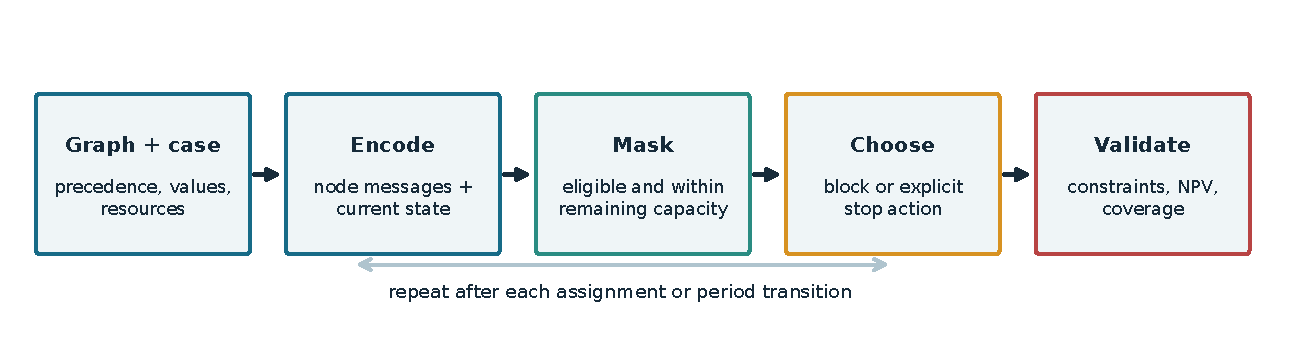
\includegraphics[width=0.98\linewidth]{figures/decision-cycle.pdf}
\caption{State-conditioned scheduling repeats graph scoring and feasibility masking after each legal assignment or period transition.}\label{fig:decision-cycle}
\end{figure}
\begin{figure}[ht]
\centering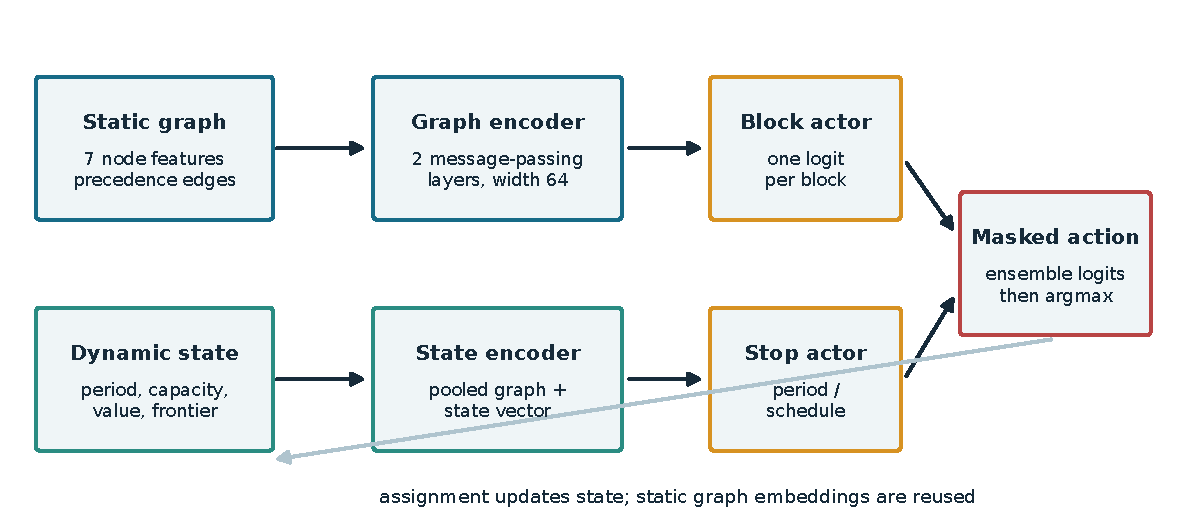
\includegraphics[width=0.9\linewidth]{figures/architecture.pdf}
\caption{The graph encoder, changing schedule state, block actor, stop actor, and masked ensemble define separate inference responsibilities.}\label{fig:architecture}
\end{figure}
\begin{figure}[ht]
\centering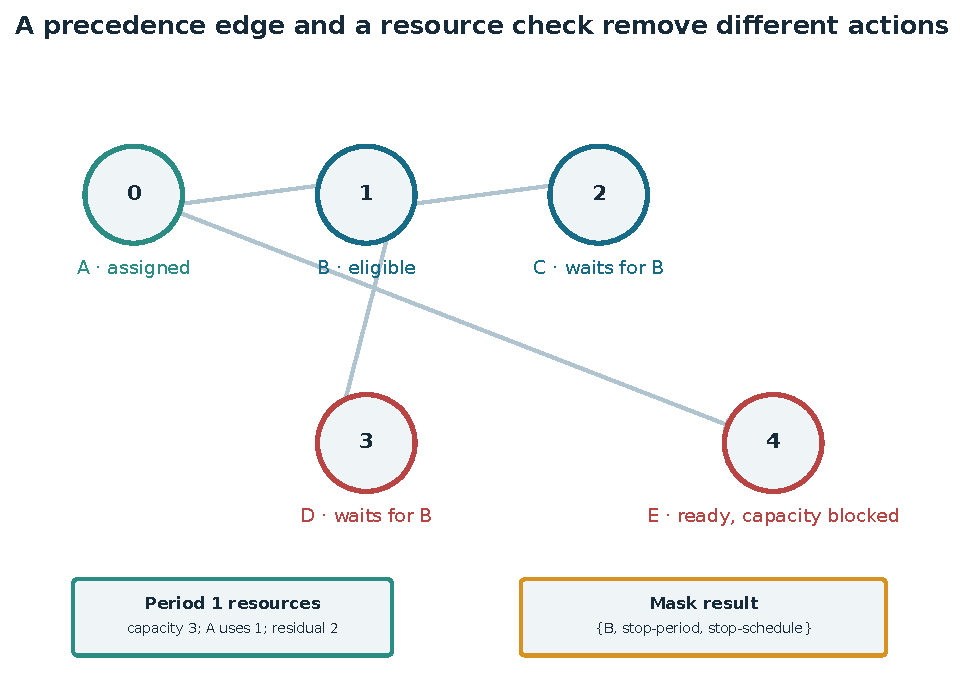
\includegraphics[width=0.82\linewidth]{figures/mask-example.pdf}
\caption{The schematic precedence graph illustrates how unmet prerequisites and insufficient residual resources exclude different blocks.}\label{fig:mask-example}
\end{figure}
\begin{figure}[ht]
\centering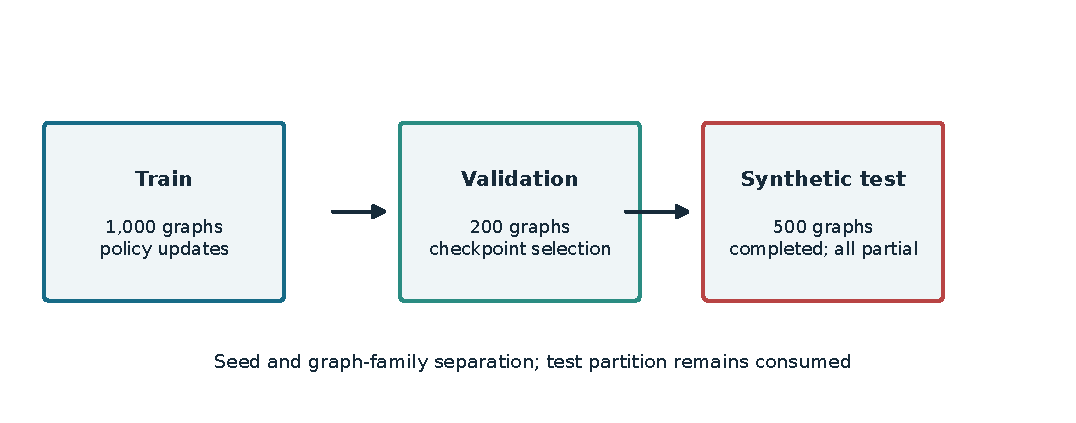
\includegraphics[width=0.88\linewidth]{figures/split-design.pdf}
\caption{The frozen design separates generated training, validation, and test partitions, while the test output loss consumes its cases.}\label{fig:split-design}
\end{figure}
\begin{figure}[ht]
\centering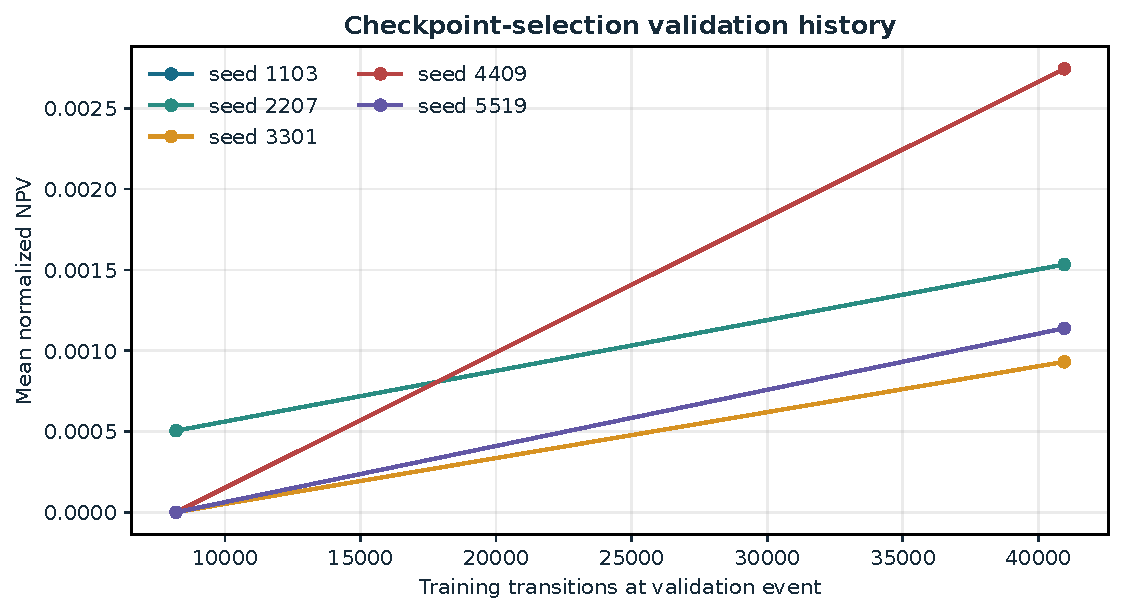
\includegraphics[width=0.8\linewidth]{figures/validation-history.pdf}
\caption{Saved checkpoint-selection events show final normalized objectives for five learner seeds; these are training-validation observations.}\label{fig:validation-history}
\end{figure}
\begin{figure}[ht]
\centering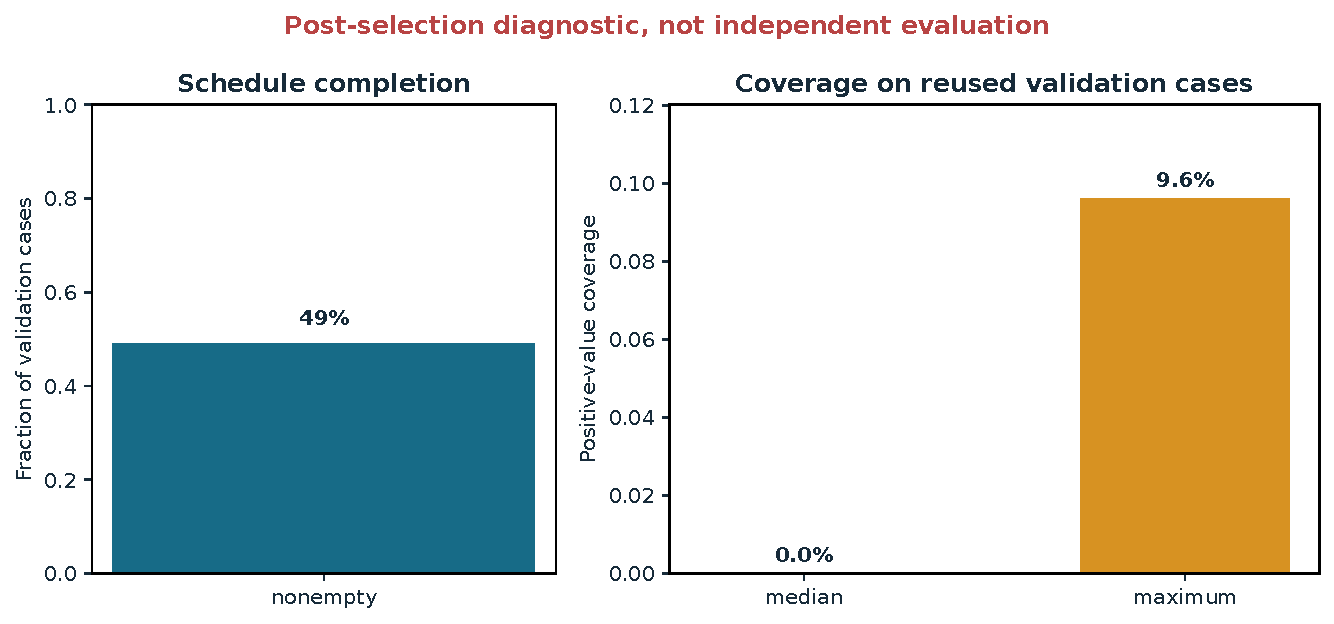
\includegraphics[width=0.82\linewidth]{figures/validation-replay.pdf}
\caption{A post-selection replay of 200 validation cases shows sparse schedules and low value coverage without an independent test claim.}\label{fig:validation-replay}
\end{figure}
\begin{figure}[ht]
\centering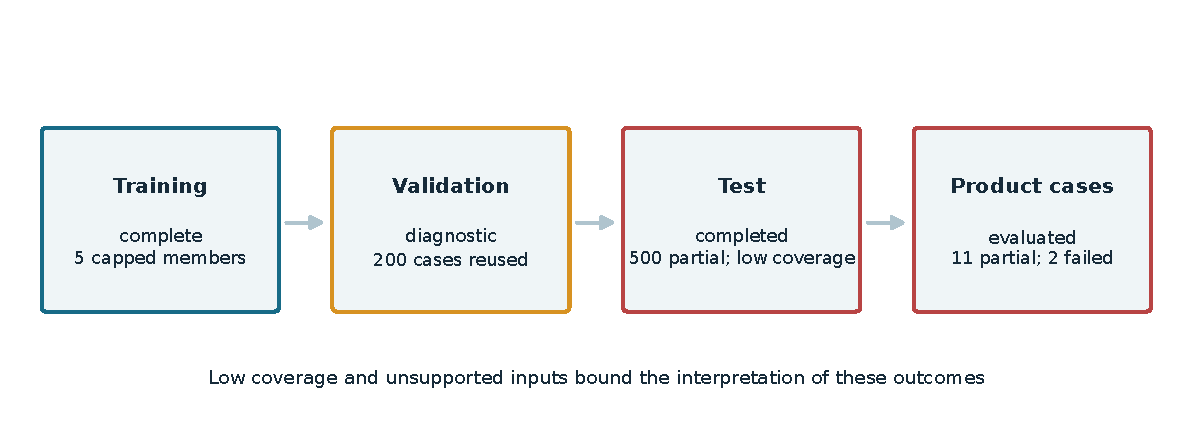
\includegraphics[width=0.92\linewidth]{figures/evidence-boundary.pdf}
\caption{Training and validation diagnostics survived, but the synthetic test outputs were lost and product cases remain unopened.}\label{fig:evidence-boundary}
\end{figure}
\begin{figure}[ht]
\centering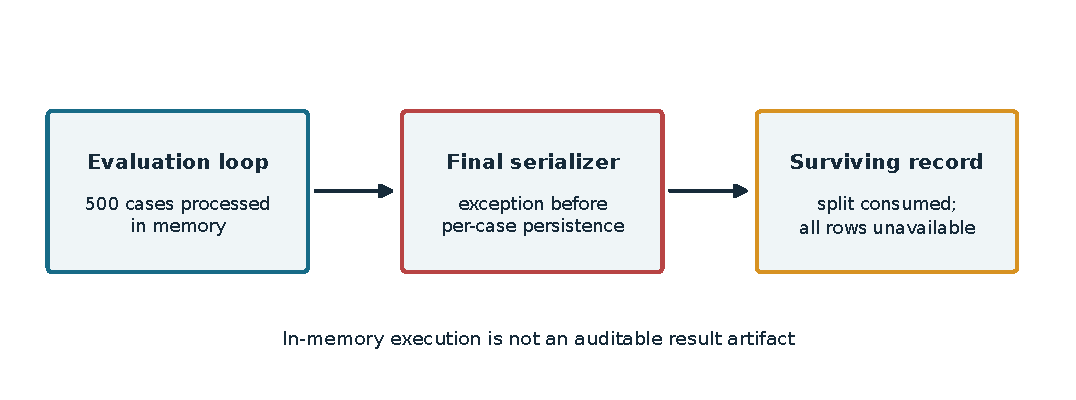
\includegraphics[width=0.88\linewidth]{figures/failure-path.pdf}
\caption{The one-shot evaluator processed cases in memory before final serialization failed and left all test outcomes unavailable.}\label{fig:failure-path}
\end{figure}

\clearpage
\raggedright
\begin{thebibliography}{99}
\bibitem{lerchs1965} H. Lerchs and I. F. Grossmann, ``Optimum design of open-pit mines,'' \emph{Transactions of the Canadian Institute of Mining and Metallurgy}, 58, 47--54, 1965.
\bibitem{picard1976} J.-C. Picard, ``Maximal closure of a graph and applications to combinatorial problems,'' \emph{Management Science}, 22(11), 1268--1272, 1976. doi:10.1287/mnsc.22.11.1268.
\bibitem{hochbaum2004} D. S. Hochbaum, ``50th anniversary article: Selection, provisioning, shared fixed costs, maximum closure, and implications on algorithmic methods today,'' \emph{Management Science}, 50(6), 709--723, 2004. doi:10.1287/mnsc.1040.0242.
\bibitem{espinoza2013} D. Espinoza, M. Goycoolea, E. Moreno, and A. Newman, ``MineLib: A library of open pit mining problems,'' \emph{Annals of Operations Research}, 206(1), 93--114, 2013. doi:10.1007/s10479-012-1258-3.
\bibitem{jelvez2018} E. J\'elvez, N. Morales, and P. Nancel-Penard, ``Open-pit mine production scheduling: Improvements to MineLib library problems,'' in \emph{Proceedings of the 27th International Symposium on Mine Planning and Equipment Selection}, 223--232, 2019. doi:10.1007/978-3-319-99220-4\_18.
\bibitem{chicoisne} R. Chicoisne, D. Espinoza, M. Goycoolea, E. Moreno, and E. Rubio, ``A new algorithm for the open-pit mine production scheduling problem,'' \emph{Operations Research}, 60(3), 517--528, 2012. doi:10.1287/opre.1120.1050.
\bibitem{caccetta2003} L. Caccetta and S. P. Hill, ``An application of branch and cut to open pit mine scheduling,'' \emph{Journal of Global Optimization}, 27(2--3), 349--365, 2003. doi:10.1023/A:1024835022186.
\bibitem{gershon} M. Gershon, ``Heuristic approaches for mine planning and production scheduling,'' \emph{International Journal of Mining and Geological Engineering}, 5, 1--13, 1987. doi:10.1007/BF01553529.
\bibitem{lambert2014} W. B. Lambert, A. Brickey, A. M. Newman, and K. Eurek, ``Open-pit block-sequencing formulations: A tutorial,'' \emph{Interfaces}, 44(2), 127--142, 2014. doi:10.1287/inte.2013.0731.
\bibitem{newman2010} A. M. Newman, E. Rubio, R. Caro, A. Weintraub, and K. Eurek, ``A review of operations research in mine planning,'' \emph{Interfaces}, 40(3), 222--245, 2010. doi:10.1287/inte.1090.0492.
\bibitem{meagher2014} C. Meagher, R. Dimitrakopoulos, and D. Avis, ``Optimized open pit mine design, pushbacks and the gap problem: A review,'' \emph{Journal of Mining Science}, 50(3), 508--526, 2014. doi:10.1134/S1062739114030132.
\bibitem{bienstock} D. Bienstock and M. Zuckerberg, ``Solving LP relaxations of large-scale precedence constrained problems,'' in \emph{Integer Programming and Combinatorial Optimization}, LNCS 6080, 1--14, 2010. doi:10.1007/978-3-642-13036-6\_1.
\bibitem{munoz2017} G. Mu\~noz, D. Espinoza, M. Goycoolea, E. Moreno, M. Queyranne, and O. Rivera Letelier, ``A study of the Bienstock--Zuckerberg algorithm: Applications in mining and resource constrained project scheduling,'' \emph{Computational Optimization and Applications}, 69, 501--534, 2017. doi:10.1007/s10589-017-9946-1.
\bibitem{cullenbine2011} C. Cullenbine, R. K. Wood, and A. Newman, ``A sliding time window heuristic for open pit mine block sequencing,'' \emph{Optimization Letters}, 5, 365--377, 2011. doi:10.1007/s11590-011-0306-2.
\bibitem{boland2009} N. Boland, I. Dumitrescu, G. Froyland, and A. M. Gleixner, ``LP-based disaggregation approaches to solving the open pit mining production scheduling problem with block processing selectivity,'' \emph{Computers \& Operations Research}, 36(4), 1064--1089, 2009. doi:10.1016/j.cor.2007.12.006.
\bibitem{jelvez2016} E. J\'elvez, N. Morales, P. Nancel-Penard, J. Peypouquet, and P. Reyes, ``Aggregation heuristic for the open-pit block scheduling problem,'' \emph{European Journal of Operational Research}, 249(3), 1169--1177, 2016. doi:10.1016/j.ejor.2015.10.044.
\bibitem{askari2010} H. Askari-Nasab, K. Awuah-Offei, and H. Eivazy, ``Large-scale open pit production scheduling using mixed integer linear programming,'' \emph{International Journal of Mining and Mineral Engineering}, 2, 2010. doi:10.1504/IJMME.2010.037624.
\bibitem{moreno2017} E. Moreno, M. Rezakhah, A. Newman, and F. Ferreira, ``Linear models for stockpiling in open-pit mine production scheduling problems,'' \emph{European Journal of Operational Research}, 260(1), 212--221, 2017. doi:10.1016/j.ejor.2016.12.014.
\bibitem{rezakhah2020blend} M. Rezakhah, E. Moreno, and A. Newman, ``Practical performance of an open pit mine scheduling model considering blending and stockpiling,'' \emph{Computers \& Operations Research}, 115, 104638, 2020. doi:10.1016/j.cor.2019.02.001.
\bibitem{rezakhah2020degrade} M. Rezakhah and A. Newman, ``Open pit mine planning with degradation due to stockpiling,'' \emph{Computers \& Operations Research}, 115, 104589, 2020. doi:10.1016/j.cor.2018.11.009.
\bibitem{johnson1968} T. B. Johnson, ``Optimum open pit mine production scheduling,'' Ph.D. thesis, University of California, Berkeley, 1968. doi:10.21236/AD0672094.
\bibitem{ramazan2013} S. Ramazan and R. Dimitrakopoulos, ``Production scheduling with uncertain supply: A new solution to the open pit mining problem,'' \emph{Optimization and Engineering}, 14(2), 361--380, 2013. doi:10.1007/s11081-012-9186-2.
\bibitem{goodfellow2016} R. C. Goodfellow and R. Dimitrakopoulos, ``Global optimization of open pit mining complexes with uncertainty,'' \emph{Applied Soft Computing}, 40, 292--304, 2016. doi:10.1016/j.asoc.2015.11.038.
\bibitem{lamghari2012} A. Lamghari and R. Dimitrakopoulos, ``A diversified tabu search approach for the open-pit mine production scheduling problem with metal uncertainty,'' \emph{European Journal of Operational Research}, 222(3), 642--652, 2012. doi:10.1016/j.ejor.2012.05.029.
\bibitem{lamghari2016} A. Lamghari and R. Dimitrakopoulos, ``Progressive hedging applied as a metaheuristic to schedule production in open-pit mines accounting for reserve uncertainty,'' \emph{European Journal of Operational Research}, 253(3), 843--855, 2016. doi:10.1016/j.ejor.2016.03.007.
\bibitem{blom} M. Blom, A. R. Pearce, and P. C\^ot\'e, ``Long-term mine planning with large neighbourhood search,'' arXiv:2403.18213, 2024. doi:10.48550/arXiv.2403.18213.
\bibitem{kumar2021} A. Kumar and R. Dimitrakopoulos, ``Production scheduling in industrial mining complexes with incoming new information using tree search and deep reinforcement learning,'' \emph{Applied Soft Computing}, 110, 107644, 2021. doi:10.1016/j.asoc.2021.107644.
\bibitem{carvalho2023} J. P. de Carvalho and R. Dimitrakopoulos, ``Integrating short-term stochastic production planning updating with mining fleet management in industrial mining complexes: An actor-critic reinforcement learning approach,'' \emph{Applied Intelligence}, 53, 23179--23202, 2023. doi:10.1007/s10489-023-04774-3.
\bibitem{teichteil2023} F. Teichteil-K\"onigsbuch, G. Poveda, G. Gonz\'alez de Garibay Barba, T. Luchterhand, and S. Thi\'ebaux, ``Fast and robust resource-constrained scheduling with graph neural networks,'' in \emph{Proceedings of ICAPS}, 33, 623--633, 2023. doi:10.1609/icaps.v33i1.27244.
\bibitem{zhao2022} X. Zhao, W. Song, Q. Li, H. Shi, Z. Kang, and C. Zhang, ``A deep reinforcement learning approach for resource-constrained project scheduling,'' in \emph{2022 IEEE Symposium Series on Computational Intelligence}, 1226--1234, 2022. doi:10.1109/SSCI51031.2022.10022122.
\bibitem{schulman2017} J. Schulman, F. Wolski, P. Dhariwal, A. Radford, and O. Klimov, ``Proximal policy optimization algorithms,'' arXiv:1707.06347, 2017. doi:10.48550/arXiv.1707.06347.
\bibitem{kingma} D. P. Kingma and J. Ba, ``Adam: A Method for Stochastic Optimization,'' arXiv:1412.6980, 2014. doi:10.48550/arXiv.1412.6980.
\end{thebibliography}
\end{document}
